\subsection{Reduced Order Observer}
A reduced order observer is designed for estimating the angular velocities. In general, an observer is utilized in a control system if either one of two specific cases occur. If certain states in the system are not measured, an observer can estimate the unmeasured states by the means of some of the measured states. However, it is also possible to use an observer if the measured data gathered from the sensors is affected a significant amount of noise. As the observer in addition to estimating unmeasured states, also filters measurements \cite{observerfilter}. The former is the reason for using an observer in the control system.

As described earlier, the attitude model has six states. With the use of the observer, the first three states, $\vec{x}_{1:3}$ are equal to the outputs, $\vec{y}$, whereas the other three states are estimated, $\vec{\hat{x}}_{4:6}$.

In \autoref{fig:Observerdiagram1}, a diagram illustrating the setup of the attitude controller is shown. The highlighted lines is the reduced order observer are its corresponding inputs and output.
%
\begin{figure}[H]
    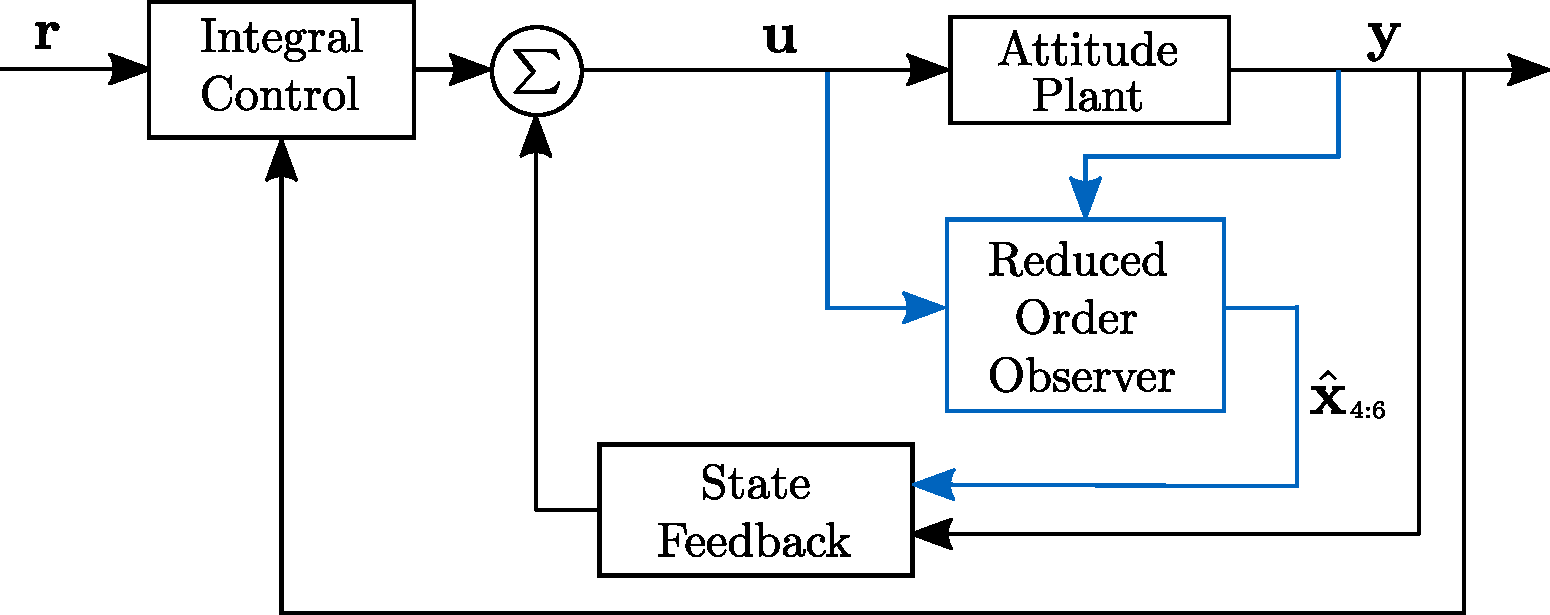
\includegraphics[scale=.4]{figures/ObserverColorDiagram}
    \centering			
    \captionof{figure}{An overall block diagram of the angular controller highlighting the reduced order observer and its corresponding inputs and output.}
    \label{fig:Observerdiagram1}
\end{figure}
%
The matrices that define the system can be separated into submatrices, which are used in the design of the observer \cite{ReducedOrderObserverChristoffer}.\\
%
\begin{minipage}{0.45\linewidth}
    \begin{flalign}
        \vec{A}=
        \begin{bmatrix}
            \ \vec{A_{11}}  & \vec{A_{12}}    \ \ \ \\ 
            \ \vec{A_{21}}  & \vec{A_{22}}    \ \ \  		
        \end{bmatrix} \nonumber
    \end{flalign}
\end{minipage}   \hfill 
\begin{minipage}{0.45\linewidth}
    \begin{flalign}
        \vec{B}=
        \begin{bmatrix}
            \ \vec{B_1}    \ \ \ \\ 
            \ \vec{B_2}     \ \ \  		
        \end{bmatrix} \nonumber
    \end{flalign}
\end{minipage}\hfill
%\begin{minipage}{0.33\linewidth}
%    \begin{flalign}
%        \vec{C}=
%        \begin{bmatrix}
%            \ \vec{C}_{3 \times 3}  & \vec{0}_{3 \times 3}  \ \ \  		
%        \end{bmatrix} \nonumber
%    \end{flalign}
%\end{minipage}

%It is thereby possible to utilize the reduced order observer theorem \fxnote{The reduced order observer theorem slide 6 course 4 control.}. This theorem states, that for an observable system there always exist an gain $L_{obs}$ which ensures that \autoref{eq:observerStable} is stable \cite{ReducedOrderObserverChristoffer}.
As the system is observable, there exists a matrix $\vec{L}_{obs}$ such that \autoref{eq:observerStable} is stable.
%
\begin{flalign}
	\vec{A_{22}} + \vec{L_{obs}}\vec{A_{12}}
		\label{eq:observerStable}
\end{flalign}
%
The observer ensures that the estimate, $\hat{x}_{4:6}$, converges to $x_{4:6}$ with a rate yielded by the eigenvalues of \autoref{eq:observerStable} \cite{ReducedOrderObserverChristoffer}.
%
\begin{flalign}
	%\vec{\dot{\hat{x}}_{4:6}} &= \vec{A}_{21}\vec{y} + \vec{A}_{22}\vec{\hat{x}_{4:6}} + \vec{B_2u} + \vec{L_{obs}}\vec{(A_{12}\hat{x}_2} - \vec{A_{21}x_2})
	\vec{\dot{\hat{x}}_{4:6}} + \vec{L}_{\mathrm{obs}}\dot{y} &= (\vec{A}_{22}+\vec{L}_{\mathrm{obs}}\vec{A}_{12})\vec{\hat{x}}_{4:6}+(\vec{A}_{21}+\vec{L}_{\mathrm{obs}}\vec{A}_{11})\vec{y}+(\vec{B}_2+\vec{L}_{\mathrm{obs}}\vec{B}_1)\vec{u}
		\label{eq:eqobservertheorem}
\end{flalign}
%
To calculate an appropriate observer gain, $L_{obs}$, it is necessary to evaluate the reliability of the utilized sensor and the model, while also taking into account the sampling rate and system delay. This is done through the different simulations shown in \autoref{sec:AttSim}.

%The matrix in \autoref{Matrix:Lobs} is the decided observer gains utilized in the reduced order observer.
%
%\begin{flalign}
%	\vec{L_{obs}} = 
%	\begin{bmatrix}
%	\ -50 & 0 & 0  \ \ \ \\ 
%	\ 0 & -60 & 0  \ \ \ \\ 
%	\ 0 & 0 & -70  \ \ \  
%	\end{bmatrix}
%	\label{Matrix:Lobs}
%\end{flalign}
%
This estimation is also shown in the form of a block diagram, \autoref{fig:observerDiagram}.
\begin{figure}[H]
	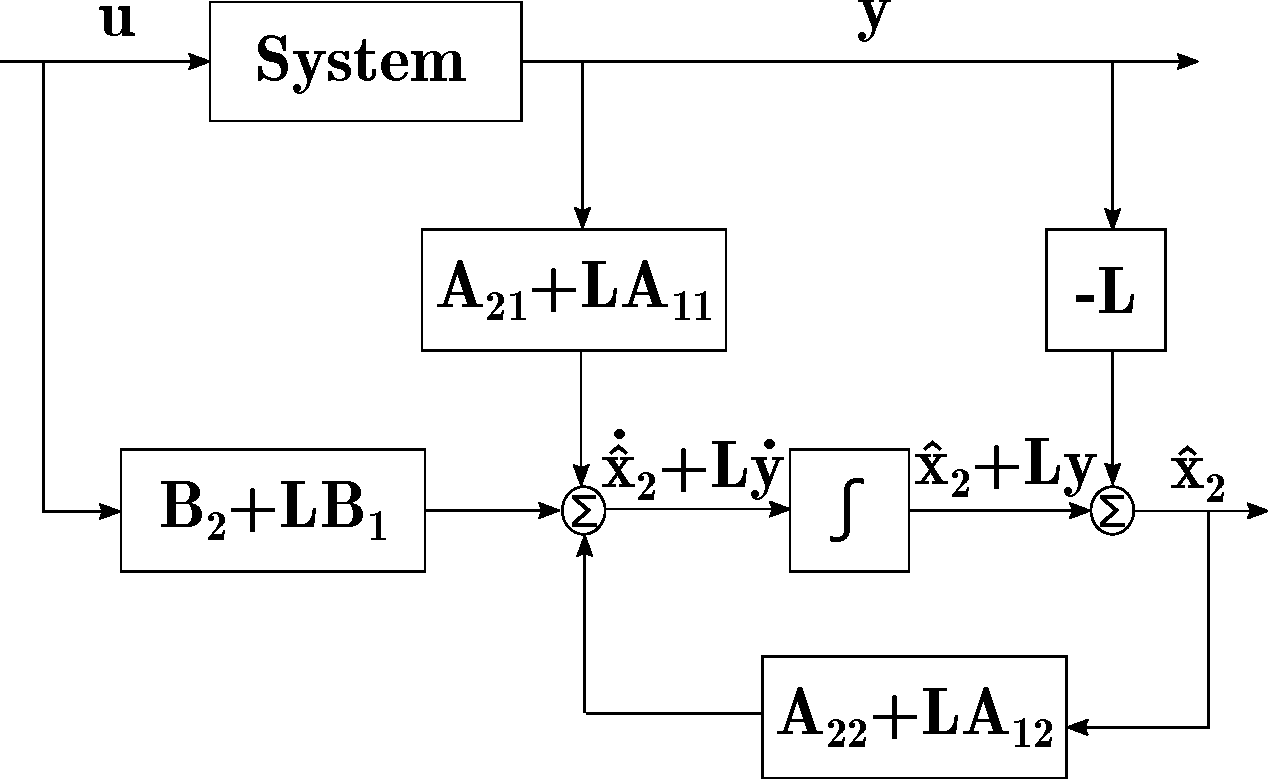
\includegraphics[scale=.35]{figures/observerDiagram}
	\centering
	\captionsetup{justification=centering}
	\captionof{figure}{A diagram showing the reduced order observer and how it is implemented.}
	\label{fig:observerDiagram}
\end{figure}
%

%\begin{minipage}{0.15\linewidth}
%	\begin{flalign}
%	A_{11} = 
%	\begin{bmatrix}
%		\ 0 & 0 & 0 \ \ \\ 
%		\ 0 & 0 & 0 \ \ \\ 
%		\ 0 & 0 & 0 \ \ \\
%	\end{bmatrix}	\nonumber
%	\label{A11}
%	\end{flalign}  
%\end{minipage}\hfill
%\begin{minipage}{0.15\linewidth}
%	\begin{flalign}
%	A_{12} = 
%	\begin{bmatrix}
%		\ 1 & 0 & 0 \ \ \\ 
%		\ 0 & 1 & 0 \ \ \\ 
%		\ 0 & 0 & 1 \ \ \\
%	\end{bmatrix}	\nonumber
%	\label{A12}
%	\end{flalign}
%\end{minipage}\hfill
%\begin{minipage}{0.15\linewidth}
%	\begin{flalign}
%	A_{21} = 
%	\begin{bmatrix}
%		\ 0 & 0 & 0 \ \ \\ 
%		\ 0 & 0 & 0 \ \ \\ 
%		\ 0 & 0 & 0 \ \ \\
%	\end{bmatrix}	\nonumber
%	\label{A21}
%	\end{flalign}
%\end{minipage}\hfill
%\begin{minipage}{0.15\linewidth}
%	\begin{flalign}
%	A_{22} = 
%	\begin{bmatrix}
%		\ 0 & 0 & 0 & 0 \ \ \\ 
%		\ 0 & 0 & 0 & 0 \ \ \\ 
%		\ 0 & 0 & 0 & 0 \ \ \\
%	\end{bmatrix} \nonumber
%	\label{A22}
%	\end{flalign}
%\end{minipage}\hfill
%
%
%\begin{minipage}{0.4\linewidth}
%	\begin{flalign}
%	B_1 = 
%	\begin{bmatrix}
%		\ 0 & 0 & 0 & 0 \ \ \\ 
%		\ 0 & 0 & 0 & 0 \ \ \\ 
%		\ 0 & 0 & 0 & 0 \ \ \\
%	\end{bmatrix}	\nonumber
%	\label{B1}
%	\end{flalign}
%\end{minipage}\hfill
%\begin{minipage}{0.6\linewidth}
%	\begin{flalign}
%	B_2 = 
%	\begin{bmatrix}
%		0 & \si{-\frac{2 \  k_{th} \  L \  \overline{\omega}_2}{J_x}} & 0 & \si{\frac{2 \  k_{th} \  L \  \overline{\omega}_4}{J_x}} \ \ \ \\ 
%		\ \si{\frac{2 \  k_{th} \  L \  \overline{\omega}_1}{J_y}} & 0 & \si{-\frac{2 \  k_{th} \  L \  \overline{\omega}_3}{J_y}} & 0 \ \ \ \\ 
%		\frac{2 \  k_d \  {\overline{\omega}_1}}{J_z} & - \frac{2 \  k_d \  {\overline{\omega}_2}}{J_z} & \frac{2 \  k_d \  {\overline{\omega}_3}}{J_z} & - \frac{2 \  k_d \  {\overline{\omega}_4}}{J_z} \ \ \
%	\end{bmatrix} \nonumber
%	\label{B2}
%	\end{flalign}
%\end{minipage}\hfill
%
%
%\begin{flalign}
%	L_{obs} = 
%	\begin{bmatrix}
%	\ -50 & 0 & 0  \ \ \ \\ 
%	\ 0 & -60 & 0  \ \ \ \\ 
%	\ 0 & 0 & -70  \ \ \  
%	\end{bmatrix}
%	\label{Lobs}
%\end{flalign}